\documentclass[12pt]{article}
\usepackage{tikz}

\usepackage{graphicx, titling, amsmath, amsthm, amsfonts, amssymb, algorithm, algpseudocode}
\usepackage{tikz}

\graphicspath{{./P-Value_Distribution.png/}}

\renewcommand\maketitlehooka{\null\mbox{}\vfill}
\renewcommand\maketitlehookd{\vfill\null}

\title{E0 259 - Assignment 3}
\author{Shankaradithyaa Venkateswaran\\ Sr no: 22190}
\date{\today}

\begin{document}
\begin{titlepage}
    \maketitle
\end{titlepage}

\section*{Output}
After running the code, the output is as follows:\\
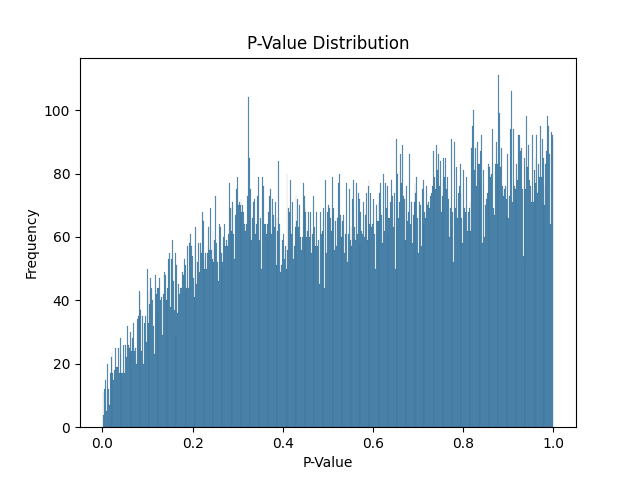
\includegraphics[width=1\textwidth]{P-Value Distribution.png}

\section*{Implementation Summary:}
I used a slew of libraries in Python to implement the code. The libraries used are:
\begin{itemize}
    \item numpy
    \item matplotlib
    \item scipy
    \item pandas
    \item seaborn
    \item math
\end{itemize}
I used pandas to read the data from the text file, and drop all rows with NaN values in the GeneSymbol and EntrezGeneId columns.\\
I manually created the N and D arrays used for the formula of 2 way ANOVA. Afterwards I converted them to numpy arrays for fast computation.\\
To compute the p values, I go through each row, get the X vector and exponentiate the values as instructed in the slides. I then convert X vector to a numpy array and apply the formula for 2 way ANOVA which is:\\
$$\frac{1/(rank(D) - rank(N))}{1/(n - rank(D))} \times (\frac{X^T(1 - N(N^TN)^{\dagger}N^T)X}{X^T(1 - D(D^TD)^{\dagger}D^T)X} - 1)$$
Then I use the scipy.stats.f.cdf function to get the p value for each row.\\
After getting the p values, I plot the histogram of the p values using seaborn and matplotlib.\\
\end{document} 